\section{二维随机变量函数的分布}
\subsection{二维离散型随机变量函数的分布}
设\((X,Y)\)是二维离散型随机变量,
且\(X\)与\(Y\)有联合分布律\begin{equation*}
	p_{ij} = P(X=x_i,Y=y_j), \quad i,j=1,2,\dotsc,
\end{equation*}
则\(Z = g(X,Y)\)有分布律\begin{equation*}
	P(Z=z_k) = \sum_{g(x_i,y_j)=z_k}{p_{ij}}.
\end{equation*}

\begin{example}
设\((X,Y)\)有二维概率分布
\begin{center}
\begin{tikzpicture}
	\draw[thick](0,0)--(4,0) (0,-4)--+(4,0);
	\draw(0,-1)--+(4,0) (1,0)--+(0,-4);
	\draw(1.5,-.5)node{0}
		(2.5,-.5)node{1}
		(3.5,-.5)node{2}
		(.5,-1.5)node{-1}
		(.5,-2.5)node{0}
		(.5,-3.5)node{1}
		(.3,-.7)node{\(X\)}
		(.7,-.3)node{\(Y\)}
		(1.5,-1.5)node{\(\tfrac{1}{12}\)}
		(2.5,-1.5)node{\(\tfrac{2}{12}\)}
		(3.5,-1.5)node{\(\tfrac{2}{12}\)}
		(1.5,-2.5)node{\(\tfrac{1}{12}\)}
		(2.5,-2.5)node{\(\tfrac{1}{12}\)}
		(3.5,-2.5)node{\(0\)}
		(1.5,-3.5)node{\(\tfrac{2}{12}\)}
		(2.5,-3.5)node{\(\tfrac{1}{12}\)}
		(3.5,-3.5)node{\(\tfrac{2}{12}\)};
\end{tikzpicture}
\end{center}
\(Z=X+Y\),\(W=\max\{X,Y\}\),求\(Z,W\)的分布律.
\begin{solution}
我们可以根据上面的二维概率分布表格计算不同\(X,Y\)取值下\(Z\)的取值:
\begin{center}
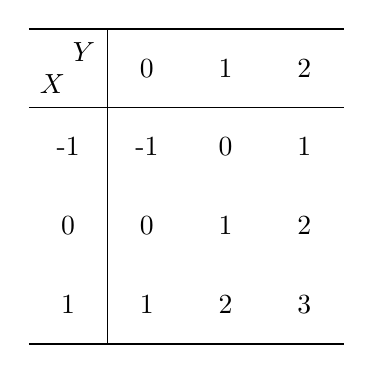
\begin{tikzpicture}
	\draw[thick](0,0)--(4,0) (0,-4)--+(4,0);
	\draw(0,-1)--+(4,0) (1,0)--+(0,-4);
	\draw(1.5,-.5)node{0}
		(2.5,-.5)node{1}
		(3.5,-.5)node{2}
		(.5,-1.5)node{-1}
		(.5,-2.5)node{0}
		(.5,-3.5)node{1}
		(.3,-.7)node{\(X\)}
		(.7,-.3)node{\(Y\)}
		(1.5,-1.5)node{-1}
		(2.5,-1.5)node{0}
		(3.5,-1.5)node{1}
		(1.5,-2.5)node{0}
		(2.5,-2.5)node{1}
		(3.5,-2.5)node{2}
		(1.5,-3.5)node{1}
		(2.5,-3.5)node{2}
		(3.5,-3.5)node{3};
\end{tikzpicture}
\end{center}
由此可知\(Z \in \Set{-1,0,1,2,3}\),那么
\def\sp#1{\sum_{x_i+y_j=#1} p_{ij}}
\begin{align*}
	&P(Z=-1) = \sp{-1} = \frac{1}{12}, \\
	&P(Z=0) = \sp{0} = \frac{1}{4}, \\
	&P(Z=1) = \sp{1} = \frac{5}{12}, \\
	&P(Z=2) = \sp{2} = \frac{1}{12}, \\
	&P(Z=3) = \sp{3} = \frac{1}{6},
\end{align*}
即\begin{equation*}
	Z \sim \begin{bmatrix}
		-1 & 0 & 1 & 2 & 3 \\
		\frac{1}{12} & \frac{1}{4} & \frac{5}{12} & \frac{1}{12} & \frac{1}{6}
	\end{bmatrix}.
\end{equation*}
同理可得,\begin{equation*}
	W \sim \begin{bmatrix}
		0 & 1 & 2 \\
		\frac{1}{6} & \frac{1}{2} & \frac{1}{3}
	\end{bmatrix}.
\end{equation*}
\end{solution}
\end{example}

\begin{theorem}\label{theorem:多维随机变量及其分布.离散型随机变量的卷积公式}
设二维离散型随机变量\((X,Y)\)有概率分布\(P(X=h,Y=k)\),
\(Z=X+Y\),则有\begin{align}
	P(Z=k)
	&= \sum_{r=0}^k P(X=r,Y=k-r) \\
	&= \sum_{r=0}^k P(X=k-r,Y=r).
\end{align}
特别地,当\(X\)与\(Y\)独立时,有\begin{align}
	P(Z=k)
	&= \sum_{r=0}^k P(X=r) \cdot P(Y=k-r) \label{equation:多维随机变量及其分布.离散型随机变量的卷积公式1} \\
	&= \sum_{r=0}^k P(X=k-r) \cdot P(Y=r). \label{equation:多维随机变量及其分布.离散型随机变量的卷积公式2}
\end{align}
\rm\cref{equation:多维随机变量及其分布.离散型随机变量的卷积公式1,%
equation:多维随机变量及其分布.离散型随机变量的卷积公式2}
称为“(离散型随机变量的)\DefineConcept{卷积公式}”.
\end{theorem}

\subsection{二维连续型随机变量函数的分布}
设\((X,Y)\)是二维连续型随机变量,且有密度函数\(f(x,y)\).
若\(g(x,y)\)是连续函数,
则\(Z = g(X,Y)\)是一维连续型随机变量.
\begin{enumerate}
	\item 首先写出\((X,Y)\)的联合密度函数.

	如果只知道\(X\)和\(Y\)的边缘密度函数,
	\(X\)与\(Y\)相互独立,
	则\((X,Y)\)的联合密度函数为\begin{equation*}
		f(x,y) = f_X(x) \cdot f_Y(y).
	\end{equation*}

	如果\(Y\)是一维离散型随机变量,
	则无法写出\((X,Y)\)的联合密度函数.

	\item 根据\(X\)和\(Y\)的取值区间,确定\(Z\)的取值区间\(R(Z)\).

	\item 对任意\(z \in R(Z)\),
	求\(Z\)的分布函数\(F_Z\).

	如果我们已知\((X,Y)\)的联合密度函数\(f\),
	那么求积分可得\(Z\)的分布函数为\begin{align*}
		F_Z(z) &= P(Z \leq z)
		= P(g(X,Y) \leq z)
		= P((X,Y) \in G(z)) \\
		&= \iint_{G(z)} f(x,y) \dd{x}\dd{y}.
	\end{align*}
	这里\(G(z) = \Set{ (x,y) \given g(x,y) \leq z }\).
	当\(z \notin R(Z)\)时,有\(F_Z(z)=0\)或\(F_Z(z)=1\).

	如果在第一步因为\(Y\)是一维离散型随机变量
	而未能写出\((X,Y)\)的联合密度函数,
	不论\(X\)与\(Y\)是否相互独立,
	只管应用\hyperref[equation:条件概率.全概率公式]{全概率公式}写出
	\(Z\)的分布函数\begin{align*}
		F_Z(z)
		&= P(g(X,Y) \leq z) \\
		&= P\left( g(X,Y) \leq z, \bigcup_{k=0}^\infty (Y = y_k) \right) \\
		&= \sum_{k=0}^\infty P\left( g(X,Y) \leq z, Y = y_k \right) \\
		&= \sum_{k=0}^\infty P(g(X,Y) \leq z \vert Y = y_k) \cdot P(Y = y_k).
	\end{align*}

	\item 求导得到\(Z\)的密度函数\(f_Z(z) = F'_Z(z)\).
\end{enumerate}

\begin{example}
设\((X,Y)\)的密度函数为\begin{equation*}
f(x,y) = \left\{ \begin{array}{cl}
xy, & 0 \leq x \leq 2, 0 \leq y \leq 1, \\
0, & \text{其他}.
\end{array} \right.
\end{equation*}求\(Z = XY\)的密度.
\begin{solution}
\begin{figure}[htb]
	\centering
	\begin{tikzpicture}
		\pgfmathsetmacro{\z}{1.5}
		\begin{axis}[
			xmin=0,xmax=2.5,
			ymin=0,ymax=2.5,
			axis lines=middle,
			axis equal=true,
			xlabel=$x$,
			ylabel=$y$,
			enlarge x limits=0.1,
			enlarge y limits=0.1,
			x label style={at={(ticklabel* cs:1.00)}, inner sep=5pt, anchor=south},
			y label style={at={(ticklabel* cs:1.00)}, inner sep=2pt, anchor=west},
			xtick={1,1.5,2},
			xticklabels={1,$z\vphantom{1}$,2},
			ytick={1,2},
		]
			\addplot[color=blue,samples=50,smooth,domain=.1:3]{\z/x};
			\draw(0,1)-|(2,0);
			\draw[dashed,black!30](\z,0)--(\z,1);
		\end{axis}
	\end{tikzpicture}
	\caption{}
	\label{figure:多维随机变量及其分布.二维连续型随机变量函数的分布.例1}
\end{figure}
由题意有,\(Z\)的值域为\(R(Z)=[0,2]\).
如\cref{figure:多维随机变量及其分布.二维连续型随机变量函数的分布.例1},
对\(\forall z\in[0,2]\),有\begin{align*}
	F_Z(z) &= P(Z \leq z)
	= P(XY \leq z)
	= \iint_{xy \leq z} f(x,y) \dd{x}\dd{y} \\
	&= \int_0^z \dd{x} \int_0^1 xy \dd{y}
		+ \int_z^2 \dd{x} \int_0^{z/x} xy \dd{y} \\
	&= \frac{z^2}{4} + \frac{z^2}{2} (\ln2 - \ln z),
\end{align*}
于是\begin{equation*}
	f_Z(z) = F_Z'(z)
	= \left\{ \begin{array}{cl}
		z \ln(2/z), & 0<z\leq2, \\
		0, & \text{其他}.
	\end{array} \right.
\end{equation*}
\end{solution}
\end{example}

\begin{example}
%@see: 《2009年全国硕士研究生入学统一考试(数学一)》一选择题/第8题
设随机变量\(X\)与\(Y\)相互独立,
且\(X\)服从标准正态分布\(N(0,1)\),
\(Y\)的概率分布为\(P(Y=0) = P(Y=1) = \frac12\).
记\(F_Z\)为随机变量\(Z=XY\)的分布函数.
讨论函数\(F_Z\)的间断点个数.
\begin{solution}
易知\(Z\)的分布函数为\begin{align*}
	F_Z(z) = P(XY \leq z)
	&= P(XY \leq z \vert Y = 0) P(Y = 0)
	+ P(XY \leq z \vert Y = 1) P(Y = 1) \\
	&= \frac12 \left[ P(X\cdot0 \leq z) + P(X \leq z) \right].
\end{align*}

当\(z < 0\)时,\((X\cdot0 \leq z)\)不可能发生,故有\begin{equation*}
	F_Z(z) = \frac12 \Phi(z),
\end{equation*}
其中\(\Phi\)是标准正态分布的分布函数.

当\(z \geq 0\)时,有\begin{equation*}
	F_Z(z) = \frac12 [1 + \Phi(z)].
\end{equation*}

显然点\(z=0\)是\(F_Z\)的间断点.
\end{solution}
\end{example}

\begin{example}
设\(X \sim U(0,1)\),\(Y \sim e(1)\),且\(X\)与\(Y\)相互独立,\(Z = X+Y\).
求\(Z\)的密度函数.
\begin{solution}
由题意有,\((X,Y)\)的密度函数为\begin{equation*}
	f(x,y) = \begin{cases}
		e^{-y}, & 0<x<1,y>0, \\
		0, & \text{其他};
	\end{cases}
\end{equation*}
\(Z\)的值域为\(R(Z)=(0,+\infty)\).
对\(\forall z>0\),有\begin{align*}
	F_Z(z) &= P(Z \leq z) = P(X+Y \leq z) \\
	&= \iint_{x+y \leq z} f(x,y) \dd{x}\dd{y}.
\end{align*}
\begin{figure}
	\centering
	\begin{tikzpicture}
		\pgfmathsetmacro{\z}{2}
		\fill[black!30](0,0)--(\z,0)--(0,\z)--(0,0);
		\begin{scope}[>=Stealth,->]
			\draw(0,0)node[below left]{\(O\)}--(4,0)node[below]{\(x\)};
			\draw(0,0)--(0,4)node[left]{\(y\)};
		\end{scope}
		\draw(0,\z)--(\z,0)node[below]{\(z\)}
			node[pos=.1,above=5pt,right=5pt]{\(\begin{array}{l}
			x+y=z \\
			0<z<1
			\end{array}\)};
		\draw(3,0)node[below]{\(1\)}--(3,3);

		\begin{scope}[xshift=6cm]
		\pgfmathsetmacro{\z}{3.5}
		\fill[black!30](0,0)--(3,0)--(3,.5)--(0,0)
			(0,0)--(3,.5)--(0,3.5)--(0,0);
		\begin{scope}[>=Stealth,->]
			\draw(0,0)node[below left]{\(O\)}--(4,0)node[below]{\(x\)};
			\draw(0,0)--(0,4)node[left]{\(y\)};
		\end{scope}
		\draw(0,\z)--(\z,0)node[below]{\(z\)}
			node[pos=.1,above=5pt,right=5pt]{\(\begin{array}{l}
			x+y=z \\
			z\geq1
			\end{array}\)};
		\draw(3,0)node[below]{\(1\)}--(3,3);
		\end{scope}
	\end{tikzpicture}
	\caption{}
	\label{figure:多维随机变量及其分布.二维连续型随机变量函数的分布.例2}
\end{figure}
如\cref{figure:多维随机变量及其分布.二维连续型随机变量函数的分布.例2},
当\(0<z<1\)时,\begin{equation*}
	F_Z(z) = \int_0^z \dd{x} \int_0^{z-x} e^{-y} \dd{y}
	= \int_0^z (1-e^{x-z}) \dd{x}
	= z-1+e^{-z}.
\end{equation*}
当\(z\geq1\)时,\begin{equation*}
	F_Z(z) = \int_0^1 \dd{x} \int_0^{z-x} e^{-y} \dd{y}
	= \int_0^1 (1-e^{x-z}) \dd{x}
	= 1-e^{-z}(e-1).
\end{equation*}
于是\begin{equation*}
	f_Z(z) = F'_Z(z)
	= \begin{cases}
		1 - e^{-z}, & 0<z<1, \\
		e^{-z}(e-1), & z\geq1, \\
		0, & \text{其他}.
	\end{cases}
\end{equation*}
\end{solution}
\end{example}

\begin{example}
设\(X,Y\)独立同分布于\(U(0,1)\),\(Z=\frac{X}{Y}\),
求\(Z\)的密度函数.
\begin{solution}
由题意有,\((X,Y)\)的密度函数为\begin{equation*}
	f(x,y) = \begin{cases}
		1, & 0<x<1,0<y<1, \\
		0, & \text{其他};
	\end{cases}
\end{equation*}
\(Z\)的值域为\(R(Z)=(0,+\infty)\).
对\(\forall z>0\),有\begin{align*}
	F_Z(z) &= P(Z \leq z) = P\left(\frac{X}{Y} \leq z\right) \\
	&= \iint_{\frac{x}{y} \leq z} f(x,y) \dd{x}\dd{y}.
\end{align*}
\begin{figure}
	\centering
	\begin{tikzpicture}
		\pgfmathsetmacro{\a}{3}
		\pgfmathsetmacro{\z}{.7}
		\fill[black!30](0,0)--(\z*\a,\a)--(0,\a)--(0,0);
		\begin{scope}[>=Stealth,->]
			\draw(0,0)node[below left]{\(O\)}--(4,0)node[below]{\(x\)}
				node[midway,below=.5cm]{\(\begin{array}[t]{l}
					x=yz \\
					0<z<1
					\end{array}\)};
			\draw(0,0)--(0,4)node[left]{\(y\)};
		\end{scope}
		\pgfmathsetmacro{\pb}{1.1*\a}
		\pgfmathsetmacro{\pa}{\pb*\z}
		\draw(0,0)--(\z*\a,\a)--(\pa,\pb);
		\draw[dashed](\z*\a,0)node[below]{\(z\)}--(\z*\a,\a);
		\draw(\a,0)node[below]{\(1\)}--(\a,\a)--(0,\a)node[left]{\(1\)};

		\begin{scope}[xshift=6cm]
			\pgfmathsetmacro{\z}{1.6}
			\fill[black!30](0,0)--(\a,\a/\z)--(0,\a)--(0,0)
				(0,\a)--(\a,\a)--(\a,\a/\z)--(0,\a);
			\begin{scope}[>=Stealth,->]
				\draw(0,0)node[below left]{\(O\)}--(4,0)node[below]{\(x\)}
					node[midway,below=.5cm]{\(\begin{array}[t]{l}
					x=yz \\
					z\geq1
					\end{array}\)};
				\draw(0,0)--(0,4)node[left]{\(y\)};
			\end{scope}
			\pgfmathsetmacro{\pa}{1.1*\a}
			\pgfmathsetmacro{\pb}{\pa/\z}
			\draw(0,0)--(\a,\a/\z)--(\pa,\pb);
			\draw[dashed](0,\a/\z)node[left]{\(\frac{1}{z}\)}--(\a,\a/\z);
			\draw(\a,0)node[below]{\(1\)}--(\a,\a)--(0,\a)node[left]{\(1\)};
		\end{scope}
	\end{tikzpicture}
	\caption{}
	\label{figure:多维随机变量及其分布.二维连续型随机变量函数的分布.例3}
\end{figure}
如\cref{figure:多维随机变量及其分布.二维连续型随机变量函数的分布.例3},
当\(0<z<1\)时,\begin{equation*}
	F_Z(z)
	= \int_0^z \dd{x} \int_{\frac{x}{z}}^1 \dd{y}
	= \frac{z}{2};
\end{equation*}
当\(z\geq1\)时,\begin{equation*}
	F_Z(z)
	= \int_0^1 \dd{x} \int_{\frac{x}{z}}^1 \dd{y}
	= 1 - \frac{1}{2z}.
\end{equation*}
于是\begin{equation*}
	f_Z(z) = F'_Z(z) = \def\arraystretch{1.5} \begin{cases}
		\frac{1}{2}, & 0<z<1, \\
		\frac{1}{2z^2}, & z\geq1, \\
		0, & \text{其他}.
	\end{cases}
\end{equation*}
\end{solution}
\end{example}

\begin{example}
%@see: 《2023年全国硕士研究生入学统一考试(数学一)》三解答题/第22题(III)
设二维随机变量\((X,Y)\)的概率密度为\begin{equation*}
	f(x,y) = \left\{ \begin{array}{cl}
		\frac2\pi (x^2+y^2), & x^2+y^2\leq1, \\
		0, & \text{其他}.
	\end{array} \right.
\end{equation*}
求\(Z = X^2 + Y^2\)的概率密度.
\begin{solution}
记\(Z\)的分布函数为\(F_Z(z)\).
当\(z < 0\)时,\(F_Z(z) = 0\).
当\(z \geq 1\)时,\(F_Z(z) = 1\).
当\(0 \leq z < 1\)时,有\begin{align*}
%@Mathematica: Integrate[2/Pi Boole[x^2 + y^2 <= z] (x^2 + y^2), {x, -1, 1}, {y, -1, 1}, Assumptions -> {0 < z < 1}]
	F_Z(z) &= P(Z \leq z)
	= \iint_{x^2+y^2 \leq z} \frac2\pi (x^2+y^2) \dd{x}\dd{y} \\
	&= \frac2\pi \int_0^{2\pi} \dd{\theta} \int_0^{\sqrt{z}} r^2 \cdot r \dd{r}
	= z^2.
\end{align*}
于是\(Z\)的概率密度为\begin{equation*}
	f_Z(z) = F'_Z(z) = \left\{ \begin{array}{cl}
		2z, & 0 \leq z < 1, \\
		0, & \text{其他}.
	\end{array} \right.
\end{equation*}
\end{solution}
\end{example}

\begin{theorem}\label{theorem:多维随机变量及其分布.连续型随机变量的卷积公式}
设二维连续型随机变量\((X,Y)\)有密度函数\(f(x,y)\),
\(Z=X+Y\),则对任意\(z \in R(Z)\),有\begin{align}
f_Z(z) &= \int_{-\infty}^{+\infty} f(x,z-x) \dd{x} \\
&= \int_{-\infty}^{+\infty} f(z-y,y) \dd{y}.
\end{align}
特别地,当\(X\)与\(Y\)独立时,有\begin{align}
f_Z(z) &= \int_{-\infty}^{+\infty} f_X(x) f_Y(z-x) \dd{x} \label{equation:多维随机变量及其分布.连续型随机变量的卷积公式1} \\
&= \int_{-\infty}^{+\infty} f_X(z-y) f_Y(y) \dd{y}. \label{equation:多维随机变量及其分布.连续型随机变量的卷积公式2}
\end{align}
\rm\cref{equation:多维随机变量及其分布.连续型随机变量的卷积公式1,%
equation:多维随机变量及其分布.连续型随机变量的卷积公式2}
称为“(连续型随机变量的)\DefineConcept{卷积公式}”.
\end{theorem}

\begin{example}
\((X,Y)\)有密度函数\begin{equation*}
	f(x,y) = \begin{cases}
		2-x-y, & 0<x<1,0<y<1, \\
		0, & \text{其他}.
	\end{cases}
\end{equation*}
\(Z=X+Y\),求\(f_Z(z)\).
\begin{solution}
由题意有,\(Z\)的值域为\(R(Z)=(0,2)\).
对\(\forall z\in(0,2)\),
由\cref{theorem:多维随机变量及其分布.连续型随机变量的卷积公式},有\begin{equation*}
	f_Z(z) = \int_{-\infty}^{+\infty} f(x,z-x) \dd{x}.
\end{equation*}
其中被积函数为\begin{equation*}
	f(x,z-x)
	= 2-x-(z-x)
	= 2-z,
	\quad
	0<x<1,0<y=z-x<1.
\end{equation*}
\begin{figure}[htb]
	\centering
	\begin{tikzpicture}[scale=.6]
		\pgfmathsetmacro{\a}{3}
		\fill[black!30](0,0)--(\a,\a)--(\a,2*\a)--(0,\a)--(0,0);
		\begin{scope}[>=Stealth,->]
			\draw(0,0)node[below left]{\(O\)}
				--(2*\a,0)node[below]{\(x\)}
				node[midway,below=.5cm]{\(\begin{array}[t]{l}
					0<x<1 \\
					x<z<1+x
				\end{array}\)};
			\draw(0,0)--(0,2.5*\a)node[left]{\(z\)};
		\end{scope}
		\draw(0,0)--(1.5*\a,1.5*\a)node[pos=.8,below right]{\(x=z\)};
		\draw(0,\a)node[left]{1}--(1.5*\a,2.5*\a)node[pos=.8,below right]{\(1+x=z\)};
		\draw(\a,0)node[below]{1}--(\a,2*\a)--(0,2*\a)node[left]{2};
	\end{tikzpicture}
	\caption{}
	\label{figure:多维随机变量及其分布.二维连续型随机变量函数的分布.例4}
\end{figure}

如\cref{figure:多维随机变量及其分布.二维连续型随机变量函数的分布.例4},
画出被积函数的定义区域\(0<x<1,x<z<1+x\).

当\(0<z<1\)时,\begin{equation*}
	f_Z(z) = \int_0^z (2-z) \dd{x} = z(2-z);
\end{equation*}
当\(1\leq z<2\)时,\begin{equation*}
	f_Z(z) = \int_{z-1}^1 (2-z) \dd{x} = (2-z)^2.
\end{equation*}
因此,\begin{equation*}
	f_Z(z) = \begin{cases}
		z(2-z), & 0<z<1, \\
		(2-z)^2, & 1\leq z<2, \\
		0, & \text{其他}.
	\end{cases}
\end{equation*}
\end{solution}
\end{example}

\begin{example}
%@see: 《2024年全国硕士研究生入学统一考试(数学一)》一选择题/第10题
设随机变量\(X,Y\)相互独立,且均服从参数为\(\lambda\)的指数分布.
令\(Z=\abs{X-Y}\).
证明:\(Z\)与\(X\)同分布.
\begin{proof}
由题意有,\((X,Y)\)的联合密度函数为\begin{equation*}
	f(x,y) = \left\{ \begin{array}{cl}
		\lambda^2 e^{-\lambda (x+y)}, & x>0,y>0, \\
		0, & \text{其他}.
	\end{array} \right.
\end{equation*}
设\(F_Z\)是\(Z\)的分布函数,
记\(D = \Set{ (x,y) \given x\geq0,y\geq0 },
D_z = \Set{ (x,y) \given -z \leq x-y \leq z }\).
当\(z < 0\)时,\(D_z = \emptyset\),\(F_Z(z) = 0\).
当\(z \geq 0\)时,\(D \cap D_Z \neq \emptyset\),\begin{align*}
	F_Z(z) = P(Z \leq z)
	&= P(\abs{X-Y} \leq z)
	= P(-z \leq X-Y \leq z) \\
	&= \iint_{D_z} f(x,y) \dd{x}\dd{y}
	= \iint_{D \cap D_z} \lambda^2 e^{-\lambda (x+y)} \dd{x}\dd{y} \\
	% 区域\(D \cap D_z\)关于直线\(y=x\)对称,可以利用轮换对称性简化运算
	&= \left( \iint_{D_1} + \iint_{D_2} \right) \lambda^2 e^{-\lambda (x+y)} \dd{x}\dd{y} \\
	&= 2 \iint_{D_1} \lambda^2 e^{-\lambda (x+y)} \dd{x}\dd{y} \\
	&= 2\lambda^2 \int_0^{+\infty} e^{-\lambda y} \dd{y}
	\int_y^{y+z} e^{-\lambda x} \dd{x}
	= 1 - e^{-\lambda z}.
\end{align*}
其中\(D_1 = \Set{ (x,y) \in D \cap D_z \given x \geq y },
D_2 = D \cap D_z - D_1\),
这就说明\(Z\)也服从参数为\(\lambda\)的指数分布.
\end{proof}
%@Mathematica: f[x_, y_] := Piecewise[{{\[Lambda]^2 Exp[-\[Lambda] (x + y)], x > 0 && y > 0}}]
%@Mathematica: Integrate[f[x, y] Boole[-z <= x - y <= z && x >= 0 && y >= 0], {x, 0, +Infinity}, {y, 0, +Infinity}, Assumptions -> {z > 0, \[Lambda] > 0}] // Simplify
\end{example}
